\section{Extracting Domain Models from Textual Requirements}\label{dmodel}
Automated support for extracting domain models from requirements artefacts such as USs play a central role in effectively supporting the detection of dependencies and conflicts between user stories. Domain models are a simple way to understand the relationship between artefacts and the whole system. 

In this section, we present a comprehensive exploration of techniques that can be employed for the extraction of domain models from agile product backlogs. Furthermore, we conduct a comparative analysis of these techniques. 
\subsection{Visual Narrator: (Automated) Extraction of Conceptual Models form US} \label{vnarrator}
Visual Narrator automatically derive conceptual models from a concise and widely adopted NL notation for USs. Robeer et al. combine NLP heuristics into an algorithm that creates conceptual modes from USs. They present the Visual Narrator as a fully automated, opensource tool that implements the algorithm and generates conceptual models as Web Ontology Languages (OWL) \cite{Robeer2016}.\\ \\ 
\textbf{A Generic Conceptual Model}\\
Robeer et al. define a generic conceptual model of stories that dissects a single US and define its syntactic structure \cite{Lucassen2015}. 

The conceptual model is assembled as a UML class diagram in figure \ref{fig:cmd}. US follow a standard predefined format \cite{Wautelet2014} to capture three distinct aspects of a requirement:
\begin{itemize}
\item Who wants the functionality;
\item What functionality the end users or stakeholders want the system to provide; and 
\item Why the end users and stakeholders need this functionality (optional).
\end{itemize}
These three aspects are captured in a simple textual template to form a running sentence. Although many different templates exist, 70\% of practitioners use the template \enquote{As a \textless type of user\textgreater, I want \textless some goal\textgreater [so that \textless come reason\textgreater ]} \cite{Greer2004}. 
The conceptual model distinguishes between the \emph{role}, \emph{means} and \emph{ends} parts of a US. Each of these parts features an \emph{indicator} which delimits the three basic parts of a US. Jointly, the indicators define the \emph{template} of a user story.

The role part encompasses the role indicator and the \emph{functional} role, describing a generalized type of person \emph{who} interacts with the system. When no ambiguity exists, Robeer et al. use the term \emph{role} to denote both the full part and the \emph{functional role}. The \emph{means} consists of a \emph{subject}, a main \emph{object} of the functionality, and a \emph{main verb} describing the relationship between the subject and main object. The main object can be represented explicitly by the direct object or implicitly (\emph{e.g.}, \enquote{I want to log in} actually, refers to logging in the \emph{system}).

Robeer et al. identified three main purposes that the \emph{ends} may take: (1) clarify the means, (2) reference another user story, or (3) introduce a qualitative requirement.
\begin{figure}
\center
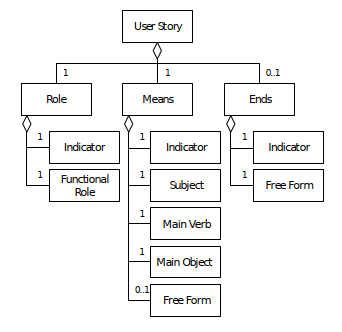
\includegraphics[width=9.03cm, height=7.76cm]{Conceptual_model_defining_the_syntax_of_a_US}
\caption{Conceptual model defining the syntax of a US  \cite{Robeer2016}}\label{fig:cmd}
\end{figure} \\  \\ 
\textbf{The Visual Narrator Tool}\\
To enable the automated extraction of conceptual modes from USs, Robeer et al. developed the \emph{Visual Narrator} tool on the basis of the 11 heuristics \cite{Robeer2016} which takes a set of USs as input and generates a conceptual model as output. The tool only accepts USs that use the indicator as identified by Wautelet \cite{Wautelet2014}: As | \emph{As a(n)} for the role, \emph{I want (to)} | \emph{I can} / \emph{I am able} / \emph{I would like} for the means, and \emph{so that} for the ends part. Syntactically invalid USs are not processed; in order to sanitize these stories, analysts should pre-process them using tools such as AQUSA \cite{lucassen2016improving}.

The architecture of Visual Narrator comprises two main components: (1) the \emph{Processor} and the (2) \emph{Constructor}. The Processor analyzes USs, parsing them into tokens using spaCy \footnote{\href{https://spacy.io/}{\emph{https://spacy.io/}}} and determining token weights based on frequency and user-defined parameters. This results in a \emph{Term-by-User-Story} matrix with weighted terms.

The Constructor then generates a conceptual model from the \emph{WeightedTokens}. It involves the \emph{PatternIdentifier}, which applies heuristics to identify patterns in USs, and the \emph{PatternFactory}, which creates an internal conceptual model based on these patterns and filters out concepts and relationships with weights below a user-specified \emph{threshold}. The Ontology component stores this model, linking parts of it to their originating USs.

To extract a conceptual model from USs, Visual Narrator implements the procedure DERIVECM which takes as input a set of raw user stories \emph{S} and empty sets of concepts \emph{C} and relationships \emph{R}, and populates $C$ and $R$ while parsing the stories and applying the 11 heuristics.

\begin{example}\label{ex_1}
The WebCompany is a young Dutch company that creates tailor-made web business applications. The team consists of nine employees who iteratively develop applications in weekly Scrum sprints. WebCompany supplied 98 user stories covering the development of an entire web application focused on interactive story telling that was created in 2014. 73 of these 98 USs were syntactically correct, usable and relevant for conceptual model generation \cite{lucassen2016improving}. Part of the generated conceptual model is shown in figure \ref{fig:webcompany}.
\begin{figure}
\center
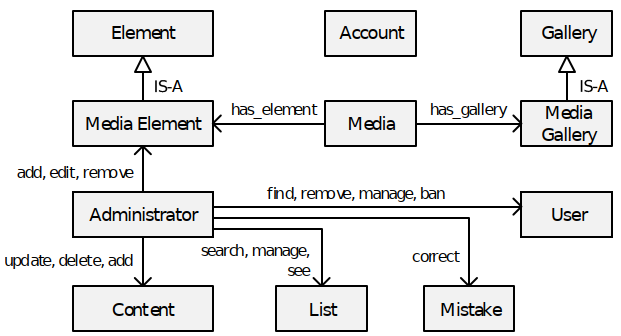
\includegraphics[width=11.03cm, height=5.76cm]{web_company}
\caption{Partial model for WebCompany generated with Visual Narrator   \cite{Robeer2016}}\label{fig:webcompany}
\end{figure}
\end{example} 
\subsection{A Modelling Backlog as Composable Graphs} \label{composable_graph}
Mosser et al. propose a model engineering method (and the associated tooling) to exploit a graph-based meta-modelling and compositional approach. The objective is to shorten the feedback loop between developers and POs while supporting agile development’s iterative and incremental nature. 

The tool can extract what is called a conceptual model of a backlog in an ontology-like way. The conceptual models are then used to measure USs quality by detecting ambiguities or defects in a given story \cite{mosser2022modelling}.
From a modelling point of view, Mosser et al. represents the concepts involved in the definition of a backlog in a metamodel, as depicted in figure \ref{fig:conceptual_metamodel}. Without surprise, the key concept is the notion of story, which brings a Benefit to a \emph{Persona} thanks to an Action performed on an \emph{Entity}. A Story is associated to a readiness \emph{Status}, and might optionally contribute to one or more \emph{QualityProperty} (\emph{e.g.}, security, performance).
\begin{figure}
\center
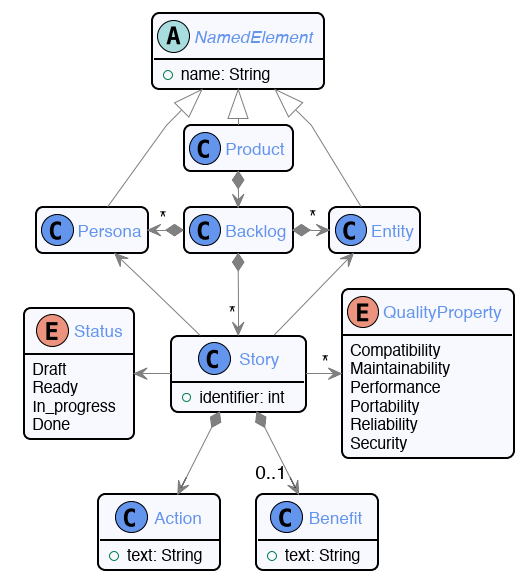
\includegraphics[width=8.03cm, height=8.76cm]{Backlog_conceptual_metamodel}
\caption{Backlog conceptual metamodel \cite{mosser2022modelling}}\label{fig:conceptual_metamodel}
\end{figure}

Consider, for example, the following story, extracted from the reference dataset \cite{Dalpiaz2018}: \enquote{As a user, I want to click on the address so that it takes me to a new tab with Google Maps.}. \emph{This story brings to the user (Persona) the benefit of reaching a new Google Maps tab (Benefit) by clicking (Action) on the displayed address (Entity).}

As Entities and Personas implement the \emph{jargon} to be used while specifying features in the backlog, they are defined at the \emph{Backlog level}. On the contrary, Actions belong to the associated stories and are not shared with other stories. Finally, a \emph{Product} is defined as the \emph{Backlog} used to specify its features.

Mosser et al. propose in the context of backlog management a system which represented in figure \ref{fig:early_feedback} is proposed for utilization. Building upon the efficiency of NLP approaches. Mosser et al. suggest employing an NLP-based extractor to create a backlog model. This model will subsequently assist teams in the planning phase by aiding in the selection of stories for implementation during the upcoming iteration \cite{mosser2022modelling}.
\begin{figure}
\center
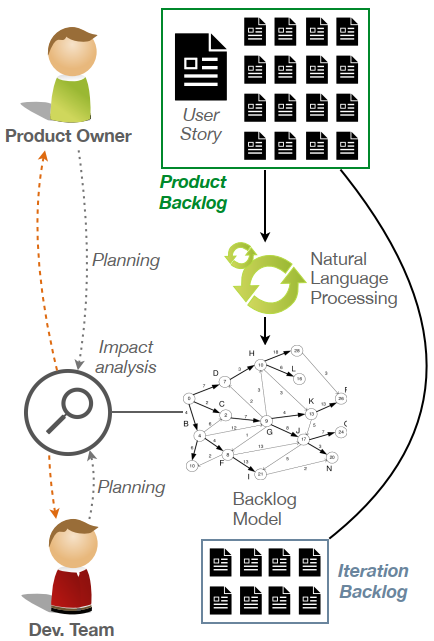
\includegraphics[width=6.03cm, height=8.76cm]{Providing_early_feedback_at_the_backlog_level}
\caption{Providing early feedback at the backlog level \cite{mosser2022modelling}}\label{fig:early_feedback}
\end{figure}\\
\textbf{Composable Backlogs}\\
In order to support team customization (\emph{e.g.}, a given team might want to enrich the backlog metamodel with additional information existing in their product management system) Mossser et al. chose open-world(ontological) representation by modelling backlog as graphs \cite{mosser2022modelling}. The graph is equipped with constraints (\emph{e.g.}, a story always refers to a persona and an entity) to ensure that the minimal structure captured in the previously defined metamodel is guaranteed.
\begin{definition}[\textbf{Story}]
A Story$s \in S$ is defined as a tuple $\left(P,A,E,K\right)$, where $P=\{p_1, ..., p_i\}$ is the set of involved personas, $A= \{a_1, ..., a_i\}$ the set of performed actions, and $E = \{e_1, ..., e_k\}$ the set of targeted entities. Additional knowledge (e.g., benefit, architectural properties, status) can be declared as key-value pairs in $K = \{(k_1,v_1), ..., (k_l,v_l)\}$. The associated semantics is that the declared actions bind personas to entities. Considering that story independence is a pillar of agile methods (as, by definition, stories are independent inside a backlog), there is no equivalence class defined over \\
$S: \forall (s,s')\in S^2, s\neq s' \Rightarrow s \not \equiv s'$.
\end{definition}
\begin{definition}[\textbf{Backlog}]
A backlog $b \in B$ is represented as an attributed typed graph $b = (V, E, A)$, with $V$ a set of typed vertices, $E$ a set of undirected edges linking existing vertices, and $A$ a set of key-value attributes. Vertices are typed according to the model element they represent $v \in V, type(v) \in \{ Persona, Entity, Story \} )$ . Edges are typed according to the kind of model elements they are binding. Like backlogs, vertices and edges can contain attributes, represented as \emph{(key, value)} pairs. The empty backlog is denoted as $\emptyset = (\emptyset ,\emptyset ,\emptyset )$.
\end{definition}
\begin{example}\label{ex_2}
Backlog excerpt: Content Management System for Cornell University — CulRepo \emph{\cite{Dalpiaz2018}}.
\begin{itemize}
\item $s_1$: As a faculty member, I want to access a collection within the repository.
\end{itemize}
Associated model:
\begin{itemize}
\item $s_1 = (\{ faculty member \} ,\{ access\} ,\{ repository, collection\} ,\emptyset)\in S$
\end{itemize}
A backlog containing a single story $s_1$: (\enquote{As a faculty member, I want to access a collection within the repository}). \\ \\ 
$b_1=\left(V_1 , E_1,\emptyset \right ) \in B$ \\ 
$V_1=\left \{ Persona(faculty \ member, \emptyset \right )$ ,

\ \ \ \ $Stroy \left (s_1, \{ \left (action, access \right ) \} \right )$

\ \ \ \ $Entity \left (repository, \emptyset \right ) $,

\ \ \ \ $Entity(collection, \emptyset ) \} $ \\ 
$E_1 = \{ has\_for\_persona(s_1,faculty \ member)$,

\ \ \ \ $has\_for\_entity \left (s_1,repository \right )$

\ \ \ \ $has\_for\_entity(s_1, collection)\}$
\end{example}
\textbf{Conditional Random Fields (CRF)} \\ 
CRFs \cite{Lafferty2001} are a particular class of \emph{Markov Random Fields}, a statistical modelling approach supporting the definition of discriminative models. They are classically used in pattern recognition tasks (labelling or parsing) when context is important identify such patterns \cite{arulmohan2023extracting}.

To apply CRF Mosser et al. transform a given story into a sequence of tuples. Each tuple contains minimally three elements: \emph{(i)} the original word from the story, \emph{(ii)} its syntactical role in the story, and \emph{(iii)} its semantical role in the story. The syntactical role in the sentence is classically known as \emph{Part-of-Speech} (POS), describing the grammatical role of the word in the sentence. The semantical role plays a dual role here. For training the model, the tags will be extracted from the annotated dataset and used as target. When used as a predictor after training, these are the data Mosser et al. will ask the model for infer.

The main limitations of CRF are that \emph{(i)} it works at the word level (model elements can spread across several words), and \emph{(ii)} it is not designed to identify relations between entities \cite{arulmohan2023extracting}.
    To address the first limitation, Mosser et al. use a glueing heuristic. Words that are consecutively associated with the same label are considered as being the same model element, \emph{e.g.}, the subsequence [\enquote{UI}, \enquote{designer}] from the previous example is considered as one single model element of type \emph{Persona}.
    
Mooser et al. applied this heuristic to everything but verbs, as classically, two verbs following each other represent different actions. They used again heuristic approach to address the second limitation. Mooser et al. bound every \emph{Persona} to every primary \emph{Action} (as\emph{ trigger} relations), and every primary \emph{Actions} to every primary \emph{Entity} (as \emph{target} relations) \cite{arulmohan2023extracting}.
\begin{example} Consider the following example:\\ \\
$S=[^\prime As^\prime,^\prime a^\prime,^\prime UI^\prime,^\prime designer^\prime,^\prime,^\prime,\ .\ .\ .]$ \\
$POS(S)=[ADP,DET,NOUN,NOUN,PUNCT,.\ .\ .]$ \\
$Label \left (S \right ) = \left [ \emptyset ,\emptyset ,PERSONA,PERSONA,\emptyset ,.\ .\ .\right ]$ \\\\
$S$ represents a given US (Table \ref{tb:feature_sets}). $POS \left (S \right )$ represent the Part-of-speech analysis of $S$. The story starts with an adposition (ADP), followed by determiner (DET), followed by a noun, followed by another noun, .... Then, $Lables\left (S \right )$ represents what we interest in: the first two words are not interesting, but the $3^{rd}\  and \ 4^{td}$ words represent a Persona.\\ 
\emph{A complete version of the example is provided in Table \ref{tb:feature_sets}.}
\end{example}
\begin{figure}
\center
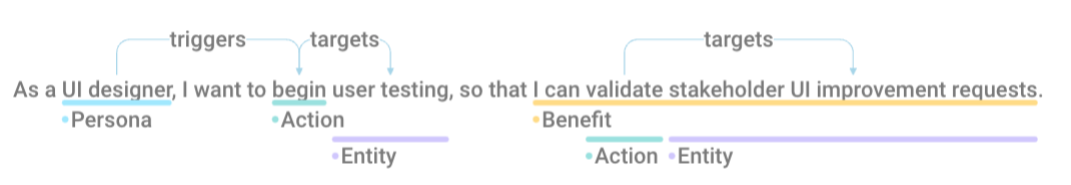
\includegraphics[width=\textwidth, height=2.76cm]{Example_of_annotated_user}
\caption{Example of annotated user using Doccano Annotation UI \cite{arulmohan2023extracting}}\label{fig:annot_usr}
\end{figure}
\begin{figure}
\begingroup
\footnotesize
\begin{tabularx}{\textwidth}{c@{\hspace{4pt}} | c@{\hspace{4pt}}  c@{\hspace{4pt}}  c@{\hspace{4pt}}  c@{\hspace{4pt}}  c@{\hspace{4pt}}  c@{\hspace{4pt}}  c@{\hspace{4pt}}  c@{\hspace{4pt}}  c@{\hspace{4pt}}  c@{\hspace{4pt}}  c@{\hspace{4pt}}  c@{\hspace{4pt}}}
Word &As &a&\textcolor[rgb]{1.0, 0.0, 0.5}{UI}&\textcolor[rgb]{1.0, 0.0, 0.5}{designer}&, &I &want &to&\textcolor[rgb]{0.21, 0.46, 0.53}{begin}&\textcolor[rgb]{0.8, 0.33, 0.0}{user} &\textcolor[rgb]{0.8, 0.33, 0.0}{testing}&,\\
POS&	ADP&	DET	&\textcolor[rgb]{1.0, 0.0, 0.5}{NOUN}	&\textcolor[rgb]{1.0, 0.0, 0.5}{NOUN}	&PUNCT	&PRON	&VERB	&PART	&\textcolor[rgb]{0.21, 0.46, 0.53}{VERB}	&\textcolor[rgb]{0.8, 0.33, 0.0}{NOUN}	&\textcolor[rgb]{0.8, 0.33, 0.0}{NOUN}	&PUNCT \\
Label	&-	&-	&\textcolor[rgb]{1.0, 0.0, 0.5}{PER}	&\textcolor[rgb]{1.0, 0.0, 0.5}{PER}	&-	&-	&-	&-	&\textcolor[rgb]{0.21, 0.46, 0.53}{P-ACT}	&\textcolor[rgb]{0.8, 0.33, 0.0}{P-ENT}	&\textcolor[rgb]{0.8, 0.33, 0.0}{P-ENT}	&- \\
 \end{tabularx}
  \begin{tabularx}{\textwidth}{c}
  \\
  \end{tabularx}
 \begin{tabularx}{\textwidth}{c@{\hspace{4pt}} | c@{\hspace{4pt}}  c@{\hspace{4pt}}  c@{\hspace{4pt}}  c@{\hspace{4pt}}  c@{\hspace{4pt}}  c@{\hspace{4pt}}  c@{\hspace{4pt}}  c@{\hspace{4pt}}  c@{\hspace{4pt}}  c@{\hspace{4pt}}  c@{\hspace{4pt}}  c@{\hspace{4pt}}}
Word&	so	&that	&I	&can	&\textcolor[rgb]{0.09, 0.45, 0.27}{validate}	&\textcolor[rgb]{0.5, 0.0, 0.5}{stakeholder}	&\textcolor[rgb]{0.5, 0.0, 0.5}{UI}	&\textcolor[rgb]{0.5, 0.0, 0.5}{improvement}	&\textcolor[rgb]{0.5, 0.0, 0.5}{requests}	&. \\
POS	&SCONJ	&SCONJ	&PRON	&AUX	&\textcolor[rgb]{0.09, 0.45, 0.27}{VERB}	&\textcolor[rgb]{0.5, 0.0, 0.5}{NOUN}	&\textcolor[rgb]{0.5, 0.0, 0.5}{NOUN}	&\textcolor[rgb]{0.5, 0.0, 0.5}{NOUN}	&\textcolor[rgb]{0.5, 0.0, 0.5}{NOUN}	&PUNCT\\
Label	&-	&-	&-	&-	&\textcolor[rgb]{0.09, 0.45, 0.27}{S-ACT}	&\textcolor[rgb]{0.5, 0.0, 0.5}{S-ENT}	&\textcolor[rgb]{0.5, 0.0, 0.5}{S-ENT}	&\textcolor[rgb]{0.5, 0.0, 0.5}{S-ENT}	&\textcolor[rgb]{0.5, 0.0, 0.5}{S-ENT}	&-\\
 \end{tabularx} \\ \\ 
\scriptsize \emph{POS tags are the Universal POS tags \\ 
Labels: PER (Persona), P-ACT (Primary Action), P-ENT (Primary Entity), S-ACT (Secondary Action), S-ENT (Secondary Entity)}
\begin{TableCaption}
\caption{Minimal Feature Set, associating part-of-speech (POS) and semantic labels to each word in a given story \cite{arulmohan2023extracting}}\label{tb:feature_sets}
\end{TableCaption}
\endgroup
\end{figure}
\subsection{Extracting Domain Models with GPT 3.5} \label{sec_gpt}
Mooser et al. experimented with ChatGPT to find the best way to extract the information from a US backlog in a \emph{\enquote{rapid prototyping}} way. They initially used a batch approach to extract information from stories using a GPT agent. However, they faced limitations due to token limits and hallucinations. To address this, they switched to a one-by-one story approach, reducing hallucinations but still producing unusable results. 

They then explored function calls introduced in \emph{gpt-3.5-turbo-0613} \footnote{\href{https://platform.openai.com/docs/guides/gpt/completions-api}{https://platform.openai.com/docs/guides/gpt/completions-api}}, allowing control over output which make developer able to provide a JSON schema in order to model their response, and the system will use this schema and \emph{\enquote{fill in the blanks}} instead of regular text generation.
\begin{example}
If one expects their answer to be an array of strings containing the name of the personas, they can provide a schema inside their request, and GPT will use it as output format (as in Figure \ref{fig:calling_gpt}, line $3 \rightarrow  12$). An example of such a constrained response is described in Figure \ref{fig:gpt_answer}.
\begin{figure}
\begin{lstlisting}[language=json,firstnumber=1]
response = openai.ChatCompletion.create(
    model = "gpt-3.5-turbo-0613",
    functions = [ #constraining_GPT_with_a_schema
	{ "name": "record_elements", #Function to be called in the response
	  "description": "Record_the_elements_extracted_from_a_story",
	  "parameters": { #Signature_description
		"type": "object",
		"properties": {
		"personas": {
			"type": "array",
			"description": "The list of personas extracted from the story",
			"items": { "type": "string" }}}],
    messages = conv,
    temperature=0.0) #To_make_the_answer_deterministic_(as_much_as_possible)
\end{lstlisting}
\caption{Calling GPT 3.5 and specifying a function call argument  \cite{arulmohan2023extracting}}\label{fig:calling_gpt}
\end{figure}
\begin{figure}
\begin{lstlisting}[language=json,firstnumber=1]
{
    ...
    "choices": [{
    	"index": 0, "message": {
	 "role": "assistant", "content": null,
	 "function_call": {
	    "name": "record_elements",
          	    "arguments":
	         "{\"personas\": [\"repository manager\"]}"
    }},
 "finish_reason": "function_call"}],
    ...
}
\end{lstlisting}
\caption{Example of answer from the API (execution of Figure \ref{fig:calling_gpt})  \cite{arulmohan2023extracting}}\label{fig:gpt_answer}
\end{figure}
\end{example}
To address limitations in GPT's output format control, the Mosser et al. introduced the option to use JSON schemas in requests, allowing users to specify the desired output format. They also explored the use of function calls as responses but found it impractical due to conversation termination. Faced with this, they had two options: defining a large schema or engaging in a conversation with the model. They chose the latter, designing the processing of each story as a conversation with a smaller, dedicated schema.
Eventually, they adopted a conversation-based approach with smaller JSON schemas to process each story effectively. 
They organized the conversation into four phases:
\begin{enumerate}
\item Setup. First, the system role will be impersonated and ask the engine to adopt a persona. 
\item Concepts. The task of extracting personas, entities, actions and benefit from a story will be proceed.
\item Categorization. Given stateless of the model, it becomes necessary to inject the answer obtained from the preceding phase into the ongoing conversation. Consequently, Mooser et al. assume the role of the assistant and include a conversation entry detailing the  \textless CONCEPTS\textgreater \ obtained in the previous phase. Following the established pattern from the prior phase, Mooser et al. articulate the task using the system role, which entails categorizing primary and secondary actions and entities.
\item Relations. The final step uses the same pattern. Mosser et al. first inject the \textless CATEGORIES\textgreater \ as the assistant, and then describe the task and provide an example as the system.
\end{enumerate}


\subsection{Comparative Analysis} \label{comparative_analysis}
In this subsection we consider a comparative analysis of mentioned methodologies to discern the most suitable approach for our specific context.

In the context of evaluating three approaches (Visual Narrator, GPT-3.5, and Conditional Random Fields or CRF) for the task of domain concept extraction from a corpus of stories, it is evident that CRF emerges as a compelling choice. Here are the reasons why CRF should be chosen for our approach:
\begin{itemize}
\item Tailored Approach: Mosser et al. highlights CRF as a rule-based approach, allows for a tailored and domain-specific model. This tailored approach is crucial when dealing with complex domain-specific tasks like concept extraction. CRF can be fine-tuned by domain experts to address the specific challenges of the task.
\item Training Requirement: CRF requires training, it was trained using a classical 80/20 separation method. This training phase allows CRF to learn the patterns and relationships between domain concepts and the textual context. This training can lead to improved accuracy and relevance in domain concept extraction (Figure \ref{fig:coparing_approaches}) \cite{arulmohan2023extracting}.
\item Model Complexity: In comparison to other approaches, CRF's implementation is relatively simple, and it requires a smaller codebase. This simplicity makes it easier to manage and maintain, reducing the complexity associated with more extensive models like GPT-3.5.
\item $F-measure\ (F_1)$ : Mosser et al. measures performance using the $F_1$ score, which is particularly suitable for this task. $F_1$ considers both precision and recall, which is essential when dealing with domain concept extraction. It is well-suited for situations where false positives and false negatives have different costs \cite{arulmohan2023extracting}.
\item Superior Performance: Empirical results indicate that CRF consistently outperformed other approaches, including GPT-3.5, in all evaluation criteria. CRF achieved the highest $F_1$ scores, particularly for Persona's extraction, reaching a perfect score of 1.0 which means a perfect match (score of 0.0 means that precision or recall is null). This superior performance is indicative of CRF's effectiveness in this specific task \cite{arulmohan2023extracting}.
\item Reproducibility: CRF offers transparency and interpretability, making it easier to understand and reproduce results compared to more opaque machine learning models.
\item Concerning the Agile DevOps Paradigms: Visual Narrator keeps its conceptual model internal and exposes black-box analysis to users, dedicated to stories quality in terms of requirements engineering, for example. Thus, it does not support the DevOps team in the development, as the provided feedback focuses on the requirements expression instead of their role in the software development. CRF instead leverage the graph structure of the ontologies and exploit a graph-based meta-modelling and compositional approach to shorten the feedback loop between developers and Ops while supporting agile development’s iterative and incremental nature \cite{mosser2022modelling}.
\item Syntactic and semantic Covering: In contrast to GPT-3.5 and CRF, which consider both the syntactic and semantic aspects of US, NLP has constrained its focus solely to the syntactic structure of the US.
\end{itemize}
\begin{figure}
\center
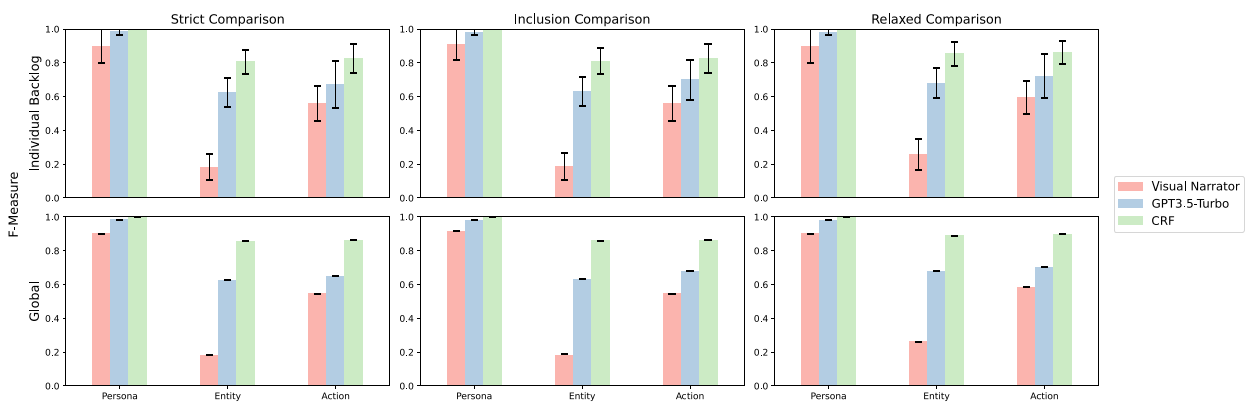
\includegraphics[width=\textwidth, height=5.76cm]{Comparing_approaches_to_the_ground_truth}
\caption{Comparing approaches to the ground truth: $F-measure \ (F_1)$ results for Visual Narrator, CRF and GPT-3.5  \cite{arulmohan2023extracting}}\label{fig:coparing_approaches}
\end{figure}
\subsection{Bottom Line}\label{crf_bottom_line}
We have chosen the Conditional Random Fields (CRF) approach because of their graph-based nature and their significant promise in terms of precision and recall, which is particularly important in the context of domain concept extraction. CRF can cover both syntactic and semantic aspects, especially when complemented by an appropriate conceptual metamodel, which makes it suitable for definition as a type graph in Henshin. The annotations generated by CRF can then be used for transformation into a rule-based graph transformation system, improving support for DevOps practices.





